\chapter{Fruitful functions}
\label{fruitchap}

\section{Return values}
\index{return value}

Some of the built-in functions we have used, such as the math
functions, produce results.  Calling the function generates a
value, which we usually assign to a variable or use as part of an
expression.

\begin{verbatim}
e = math.exp(1.0)
height = radius * math.sin(radians)
\end{verbatim}
%
All of the functions we have written so far are void; they print
something or move turtles around, but their return value is {\tt
None}.

In this chapter, we are (finally) going to write fruitful functions.
The first example is {\tt area}, which returns the area of a circle
with the given radius:

\begin{verbatim}
def area(radius):
    temp = math.pi * radius**2
    return temp
\end{verbatim}
%
We have seen the {\tt return} statement before, but in a fruitful
function the {\tt return} statement includes
an expression.  This statement means: ``Return immediately from
this function and use the following expression as a return value.''
The expression can be arbitrarily complicated, so we could
have written this function more concisely:
\index{return statement}
\index{statement!return}

\begin{verbatim}
def area(radius):
    return math.pi * radius**2
\end{verbatim}
%
On the other hand, {\bf temporary variables} like {\tt temp} often make
debugging easier.
\index{temporary variable}
\index{variable!temporary}

Sometimes it is useful to have multiple return statements, one in each
branch of a conditional:

\begin{verbatim}
def absolute_value(x):
    if x < 0:
        return -x
    else:
        return x
\end{verbatim}
%
Since these {\tt return} statements are in an alternative conditional,
only one will be executed.

As soon as a return statement executes, the function
terminates without executing any subsequent statements.
Code that appears after a {\tt return} statement, or any other place
the flow of execution can never reach, is called {\bf dead code}.
\index{dead code}

In a fruitful function, it is a good idea to ensure
that every possible path through the program hits a
{\tt return} statement.  For example:

\begin{verbatim}
def absolute_value(x):
    if x < 0:
        return -x
    if x > 0:
        return x
\end{verbatim}
%
This function is incorrect because if {\tt x} happens to be 0,
neither condition is true, and the function ends without hitting a
{\tt return} statement.  If the flow of execution gets to the end
of a function, the return value is {\tt None}, which is not
the absolute value of 0.
\index{None special value}
\index{special value!None}

\begin{verbatim}
>>> print absolute_value(0)
None
\end{verbatim}
%
By the way, Python provides a built-in function called
{\tt abs} that computes absolute values.
\index{abs function}
\index{function!abs}

\begin{exercise}
\index{compare function}
\index{function!compare}

Write a {\tt compare} function
that returns {\tt 1} if {\tt x > y},
{\tt 0} if {\tt x == y}, and {\tt -1} if {\tt x < y}.
\end{exercise}


\section{Incremental development}
\label{incremental.development}
\index{development plan!incremental}

As you write larger functions, you might find yourself
spending more time debugging.

To deal with increasingly complex programs,
you might want to try a process called
{\bf incremental development}.  The goal of incremental development
is to avoid long debugging sessions by adding and testing only
a small amount of code at a time.
\index{testing!incremental development}
\index{Pythagorean theorem}

As an example, suppose you want to find the distance between two
points, given by the coordinates $(x_1, y_1)$ and $(x_2, y_2)$.
By the Pythagorean theorem, the distance is:

\begin{displaymath}
\mathrm{distance} = \sqrt{(x_2 - x_1)^2 + (y_2 - y_1)^2}
\end{displaymath}
%
The first step is to consider what a {\tt distance} function should
look like in Python.  In other words, what are the inputs (parameters)
and what is the output (return value)?

In this case, the inputs are two points, which you can represent
using four numbers.  The return value is the distance, which is
a floating-point value.

Already you can write an outline of the function:

\begin{verbatim}
def distance(x1, y1, x2, y2):
    return 0.0
\end{verbatim}
%
Obviously, this version doesn't compute distances; it always returns
zero.  But it is syntactically correct, and it runs, which means that
you can test it before you make it more complicated.

To test the new function, call it with sample arguments:

\begin{verbatim}
>>> distance(1, 2, 4, 6)
0.0
\end{verbatim}
%
I chose these values so that the horizontal distance is 3 and the
vertical distance is 4; that way, the result is 5
(the hypotenuse of a 3-4-5 triangle). When testing a function, it is
useful to know the right answer.
\index{testing!knowing the answer}

At this point we have confirmed that the function is syntactically
correct, and we can start adding code to the body.
A reasonable next step is to find the differences
$x_2 - x_1$ and $y_2 - y_1$.  The next version stores those values in
temporary variables and prints them.

\begin{verbatim}
def distance(x1, y1, x2, y2):
    dx = x2 - x1
    dy = y2 - y1
    print 'dx is', dx
    print 'dy is', dy
    return 0.0
\end{verbatim}
%
If the function is working, it should display \verb"'dx is 3'" and {\tt
'dy is 4'}.  If so, we know that the function is getting the right
arguments and performing the first computation correctly.  If not,
there are only a few lines to check.

Next we compute the sum of squares of {\tt dx} and {\tt dy}:

\begin{verbatim}
def distance(x1, y1, x2, y2):
    dx = x2 - x1
    dy = y2 - y1
    dsquared = dx**2 + dy**2
    print 'dsquared is: ', dsquared
    return 0.0
\end{verbatim}
%
Again, you would run the program at this stage and check the output
(which should be 25).
Finally, you can use {\tt math.sqrt} to compute and return the result:
\index{sqrt}
\index{function!sqrt}

\begin{verbatim}
def distance(x1, y1, x2, y2):
    dx = x2 - x1
    dy = y2 - y1
    dsquared = dx**2 + dy**2
    result = math.sqrt(dsquared)
    return result
\end{verbatim}
%
If that works correctly, you are done.  Otherwise, you might
want to print the value of {\tt result} before the return
statement.

The final version of the function doesn't display anything when it
runs; it only returns a value.  The {\tt print} statements we wrote
are useful for debugging, but once you get the function working, you
should remove them.  Code like that is called {\bf scaffolding}
because it is helpful for building the program but is not part of the
final product.
\index{scaffolding}

When you start out, you should add only a line or two of code at a
time.  As you gain more experience, you might find yourself writing
and debugging bigger chunks.  Either way, incremental development
can save you a lot of debugging time.

The key aspects of the process are:

\begin{enumerate}

\item Start with a working program and make small incremental changes.
At any point, if there is an error, you should have a good idea
where it is.

\item Use temporary variables to hold intermediate values so you can
display and check them.

\item Once the program is working, you might want to remove some of
the scaffolding or consolidate multiple statements into compound
expressions, but only if it does not make the program difficult to
read.

\end{enumerate}

\begin{exercise}
\index{hypotenuse}

Use incremental development to write a function
called {\tt hypotenuse} that returns the length of the hypotenuse of a
right triangle given the lengths of the two legs as arguments.
Record each stage of the development process as you go.
\end{exercise}


\section{Composition}
\index{composition}
\index{function composition}

As you should expect by now, you can call one function from
within another.  This ability is called {\bf composition}.

As an example, we'll write a function that takes two points,
the center of the circle and a point on the perimeter, and computes
the area of the circle.

Assume that the center point is stored in the variables {\tt xc} and
{\tt yc}, and the perimeter point is in {\tt xp} and {\tt yp}. The
first step is to find the radius of the circle, which is the distance
between the two points.  We just wrote a function, {\tt
distance}, that does that:

\begin{verbatim}
radius = distance(xc, yc, xp, yp)
\end{verbatim}
%
The next step is to find the area of a circle with that radius;
we just wrote that, too:

\begin{verbatim}
result = area(radius)
\end{verbatim}
%
Encapsulating these steps in a function, we get:
\index{encapsulation}

\begin{verbatim}
def circle_area(xc, yc, xp, yp):
    radius = distance(xc, yc, xp, yp)
    result = area(radius)
    return result
\end{verbatim}
%
The temporary variables {\tt radius} and {\tt result} are useful for
development and debugging, but once the program is working, we can
make it more concise by composing the function calls:

\begin{verbatim}
def circle_area(xc, yc, xp, yp):
    return area(distance(xc, yc, xp, yp))
\end{verbatim}
%

\section{Boolean functions}
\label{boolean}

Functions can return booleans, which is often convenient for hiding
complicated tests inside functions.  \index{boolean function}
For example:

\begin{verbatim}
def is_divisible(x, y):
    if x % y == 0:
        return True
    else:
        return False
\end{verbatim}
%
It is common to give boolean functions names that sound like yes/no
questions; \verb"is_divisible" returns either {\tt True} or {\tt False}
to indicate whether {\tt x} is divisible by {\tt y}.

Here is an example:

\begin{verbatim}
>>>   is_divisible(6, 4)
False
>>>   is_divisible(6, 3)
True
\end{verbatim}
%
The result of the {\tt ==} operator is a boolean, so we can write the
function more concisely by returning it directly:

\begin{verbatim}
def is_divisible(x, y):
    return x % y == 0
\end{verbatim}
%
Boolean functions are often used in conditional statements:
\index{conditional statement}
\index{statement!conditional}

\begin{verbatim}
if is_divisible(x, y):
    print 'x is divisible by y'
\end{verbatim}
%
It might be tempting to write something like:

\begin{verbatim}
if is_divisible(x, y) == True:
    print 'x is divisible by y'
\end{verbatim}
%
But the extra comparison is unnecessary.

\begin{exercise}

Write a function \verb"is_between(x, y, z)" that
returns {\tt True} if $x \le y \le z$ or {\tt False} otherwise.

\end{exercise}


\section{More recursion}
\label{more.recursion}
\index{recursion}
\index{Turing complete language}
\index{language!Turing complete}
\index{Turing, Alan}
\index{Turing Thesis}

We have only covered a small subset of Python, but you might
be interested to know that this subset is a {\em complete}
programming language, which means that anything that can be
computed can be expressed in this language.  Any program ever written
could be rewritten using only the language features you have learned
so far (actually, you would need a few commands to control devices
like the keyboard, mouse, disks, etc., but that's all).

Proving that claim is a nontrivial exercise first accomplished by Alan
Turing, one of the first computer scientists (some would argue that he
was a mathematician, but a lot of early computer scientists started as
mathematicians).  Accordingly, it is known as the Turing Thesis.
For a more complete (and accurate) discussion of the Turing Thesis,
I recommend Michael Sipser's book {\em Introduction to the
Theory of Computation}.

To give you an idea of what you can do with the tools you have learned
so far, we'll evaluate a few recursively defined mathematical
functions.  A recursive definition is similar to a circular
definition, in the sense that the definition contains a reference to
the thing being defined.  A truly circular definition is not very
useful:

\begin{description}

\item[vorpal:] An adjective used to describe something that is vorpal.
\index{vorpal}
\index{circular definition}
\index{definition!circular}

\end{description}

If you saw that definition in the dictionary, you might be annoyed. On
the other hand, if you looked up the definition of the factorial
function, denoted with the symbol $!$, you might get something like
this:
%
\begin{eqnarray*}
&&  0! = 1 \\
&&  n! = n (n-1)!
\end{eqnarray*}
%
This definition says that the factorial of 0 is 1, and the factorial
of any other value, $n$, is $n$ multiplied by the factorial of $n-1$.

So $3!$ is 3 times $2!$, which is 2 times $1!$, which is 1 times
$0!$. Putting it all together, $3!$ equals 3 times 2 times 1 times 1,
which is 6.
\index{factorial function}
\index{function!factorial}
\index{recursive definition}

If you can write a recursive definition of something, you can usually
write a Python program to evaluate it. The first step is to decide
what the parameters should be.  In this case it should be clear
that {\tt factorial} takes an integer:

\begin{verbatim}
def factorial(n):
\end{verbatim}
%
If the argument happens to be 0, all we have to do is return 1:

\begin{verbatim}
def factorial(n):
    if n == 0:
        return 1
\end{verbatim}
%
Otherwise, and this is the interesting part, we have to make a
recursive call to find the factorial of $n-1$ and then multiply it by
$n$:

\begin{verbatim}
def factorial(n):
    if n == 0:
        return 1
    else:
        recurse = factorial(n-1)
        result = n * recurse
        return result
\end{verbatim}
%
The flow of execution for this program is similar to the flow of {\tt
countdown} in Section~\ref{recursion}.  If we call {\tt factorial}
with the value 3:

Since 3 is not 0, we take the second branch and calculate the factorial
of {\tt n-1}...

\begin{quote}
Since 2 is not 0, we take the second branch and calculate the factorial of
{\tt n-1}...


  \begin{quote}
  Since 1 is not 0, we take the second branch and calculate the factorial
  of {\tt n-1}...


    \begin{quote}
    Since 0 {\em is} 0, we take the first branch and return 1
    without making any more recursive calls.
    \end{quote}


  The return value (1) is multiplied by $n$, which is 1, and the
  result is returned.
  \end{quote}


The return value (1) is multiplied by $n$, which is 2, and the
result is returned.
\end{quote}


The return value (2) is multiplied by $n$, which is 3, and the result, 6,
becomes the return value of the function call that started the whole
process.
\index{stack diagram}

Figure~\ref{fig.stack3} shows what the stack diagram looks like for
this sequence of function calls.

\begin{figure}
\centerline
{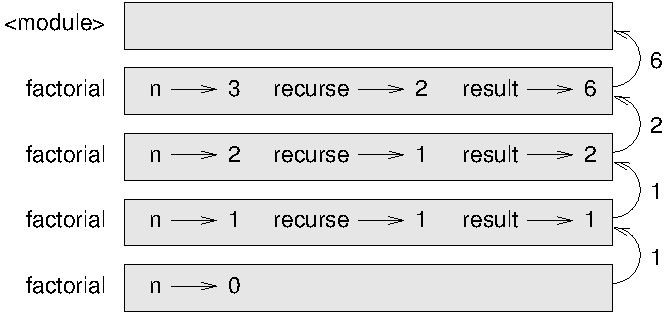
\includegraphics[scale=0.8]{figs/stack3.pdf}}
\caption{Stack diagram.}
\label{fig.stack3}
\end{figure}

The return values are shown being passed back up the stack.  In each
frame, the return value is the value of {\tt result}, which is the
product of {\tt n} and {\tt recurse}.
\index{function frame}
\index{frame}

In the last frame, the local
variables {\tt recurse} and {\tt result} do not exist, because
the branch that creates them does not execute.


\section{Leap of faith}
\index{recursion}
\index{leap of faith}

Following the flow of execution is one way to read programs, but
it can quickly become labyrinthine.  An
alternative is what I call the ``leap of faith.''  When you come to a
function call, instead of following the flow of execution, you {\em
assume} that the function works correctly and returns the right
result.

In fact, you are already practicing this leap of faith when you use
built-in functions.  When you call {\tt math.cos} or {\tt math.exp},
you don't examine the bodies of those functions.  You just
assume that they work because the people who wrote the built-in
functions were good programmers.

The same is true when you call one of your own functions.  For
example, in Section~\ref{boolean}, we wrote a function called
\verb"is_divisible" that determines whether one number is divisible by
another.  Once we have convinced ourselves that this function is
correct---by examining the code and testing---we can use the function
without looking at the body again.
\index{testing!leap of faith}

The same is true of recursive programs.  When you get to the recursive
call, instead of following the flow of execution, you should assume
that the recursive call works (yields the correct result) and then ask
yourself, ``Assuming that I can find the factorial of $n-1$, can I
compute the factorial of $n$?''  In this case, it is clear that you
can, by multiplying by $n$.

Of course, it's a bit strange to assume that the function works
correctly when you haven't finished writing it, but that's why
it's called a leap of faith!


\section{One more example}
\label{one.more.example}

\index{fibonacci function}
\index{function!fibonacci}
After {\tt factorial}, the most common example of a recursively
defined mathematical function is {\tt fibonacci}, which has the
following definition (see
  \url{http://en.wikipedia.org/wiki/Fibonacci_number}):
%
\begin{eqnarray*}
&& \mathrm{fibonacci}(0) = 0 \\
&& \mathrm{fibonacci}(1) = 1 \\
&& \mathrm{fibonacci}(n) = \mathrm{fibonacci}(n-1) + \mathrm{fibonacci}(n-2)
\end{eqnarray*}
%
Translated into Python, it looks like this:

\begin{verbatim}
def fibonacci (n):
    if n == 0:
        return 0
    elif  n == 1:
        return 1
    else:
        return fibonacci(n-1) + fibonacci(n-2)
\end{verbatim}
%
If you try to follow the flow of execution here, even for fairly
small values of $n$, your head explodes.  But according to the
leap of faith, if you assume that the two recursive calls
work correctly, then it is clear that you get
the right result by adding them together.
\index{flow of execution}


\section{Checking types}
\label{guardian}

What happens if we call {\tt factorial} and give it 1.5 as an argument?
\index{type checking}
\index{error checking}
\index{factorial function}
\index{RuntimeError}

\begin{verbatim}
>>> factorial(1.5)
RuntimeError: Maximum recursion depth exceeded
\end{verbatim}
%
It looks like an infinite recursion.  But how can that be?  There is a
base case---when {\tt n == 0}.  But if {\tt n} is not an integer,
we can {\em miss} the base case and recurse forever.
\index{infinite recursion}
\index{recursion!infinite}

In the first recursive call, the value of {\tt n} is 0.5.
In the next, it is -0.5.  From there, it gets smaller
(more negative), but it will never be 0.

We have two choices.  We can try to generalize the {\tt factorial}
function to work with floating-point numbers, or we can make {\tt
  factorial} check the type of its argument.  The first option is
called the gamma function and it's a
little beyond the scope of this book.  So we'll go for the second.
\index{gamma function}

We can use the built-in function {\tt isinstance} to verify the type
of the argument.  While we're at it, we can also make sure the
argument is positive:
\index{isinstance function}
\index{function!isinstance}

\begin{verbatim}
def factorial (n):
    if not isinstance(n, int):
        print 'Factorial is only defined for integers.'
        return None
    elif n < 0:
        print 'Factorial is not defined for negative integers.'
        return None
    elif n == 0:
        return 1
    else:
        return n * factorial(n-1)
\end{verbatim}
%
The first base case handles nonintegers; the
second catches negative integers.  In both cases, the program prints
an error message and returns {\tt None} to indicate that something
went wrong:

\begin{verbatim}
>>> factorial('fred')
Factorial is only defined for integers.
None
>>> factorial(-2)
Factorial is not defined for negative integers.
None
\end{verbatim}
%
If we get past both checks, then we know that $n$ is positive or
zero, so we can prove that the recursion terminates.
\index{guardian pattern}
\index{pattern!guardian}

This program demonstrates a pattern sometimes called a {\bf guardian}.
The first two conditionals act as guardians, protecting the code that
follows from values that might cause an error.  The guardians make it
possible to prove the correctness of the code.

In Section~\ref{raise} we will see a more flexible alternative to printing
an error message: raising an exception.


\section{Debugging}
\label{factdebug}

Breaking a large program into smaller functions creates natural
checkpoints for debugging.  \index{debugging}
If a function is not working, there are
three possibilities to consider:

\begin{itemize}

\item There is something wrong with the arguments the function
is getting; a precondition is violated.

\item There is something wrong with the function; a postcondition
is violated.

\item There is something wrong with the return value or the
way it is being used.

\end{itemize}

To rule out the first possibility, you can add a {\tt print} statement
at the beginning of the function and display the values of the
parameters (and maybe their types).  Or you can write code
that checks the preconditions explicitly.
\index{precondition}
\index{postcondition}

If the parameters look good, add a {\tt print} statement before each
{\tt return} statement that displays the return value.  If
possible, check the result by hand.  Consider calling the
function with values that make it easy to check the result
(as in Section~\ref{incremental.development}).

If the function seems to be working, look at the function call
to make sure the return value is being used correctly (or used
at all!).
\index{flow of execution}

Adding print statements at the beginning and end of a function
can help make the flow of execution more visible.
For example, here is a version of {\tt factorial} with
print statements:

\begin{verbatim}
def factorial(n):
    space = ' ' * (4 * n)
    print space, 'factorial', n
    if n == 0:
        print space, 'returning 1'
        return 1
    else:
        recurse = factorial(n-1)
        result = n * recurse
        print space, 'returning', result
        return result
\end{verbatim}
%
{\tt space} is a string of space characters that controls the
indentation of the output.  Here is the result of {\tt factorial(5)} :

\begin{verbatim}
                     factorial 5
                 factorial 4
             factorial 3
         factorial 2
     factorial 1
 factorial 0
 returning 1
     returning 1
         returning 2
             returning 6
                 returning 24
                     returning 120
\end{verbatim}
%
If you are confused about the flow of execution, this kind of
output can be helpful.  It takes some time to develop effective
scaffolding, but a little bit of scaffolding can save a lot of debugging.


\section{Glossary}

\begin{description}

\item[temporary variable:]  A variable used to store an intermediate value in
a complex calculation.
\index{temporary variable}
\index{variable!temporary}

\item[dead code:]  Part of a program that can never be executed, often because
it appears after a {\tt return} statement.
\index{dead code}

\item[{\tt None}:]  A special value returned by functions that
have no return statement or a return statement without an argument.
\index{None special value}
\index{special value!None}

\item[incremental development:]  A program development plan intended to
avoid debugging by adding and testing only
a small amount of code at a time.
\index{incremental development}

\item[scaffolding:]  Code that is used during program development but is
not part of the final version.
\index{scaffolding}

\item[guardian:]  A programming pattern that uses a conditional
statement to check for and handle circumstances that
might cause an error.
\index{guardian pattern}
\index{pattern!guardian}

\end{description}


\section{Exercises}

\begin{exercise}

Draw a stack diagram for the following program.  What does the program print?
Solution: \url{http://thinkpython.com/code/stack_diagram.py}.
\index{stack diagram}

\begin{verbatim}
def b(z):
    prod = a(z, z)
    print z, prod
    return prod

def a(x, y):
    x = x + 1
    return x * y

def c(x, y, z):
    total = x + y + z
    square = b(total)**2
    return square

x = 1
y = x + 1
print c(x, y+3, x+y)
\end{verbatim}

\end{exercise}


\begin{exercise}
\label{ackermann}

The Ackermann function, $A(m, n)$, is defined:

\begin{eqnarray*}
A(m, n) = \begin{cases}
              n+1 & \mbox{if } m = 0 \\
        A(m-1, 1) & \mbox{if } m > 0 \mbox{ and } n = 0 \\
A(m-1, A(m, n-1)) & \mbox{if } m > 0 \mbox{ and } n > 0.
\end{cases}
\end{eqnarray*}
%
See \url{http://en.wikipedia.org/wiki/Ackermann_function}.
Write a function named {\tt ack} that evaluates Ackermann's function.
Use your function to evaluate {\tt ack(3, 4)}, which should be 125.
What happens for larger values of {\tt m} and {\tt n}?
Solution: \url{http://thinkpython.com/code/ackermann.py}.
\index{Ackermann function}
\index{function!ack}

\end{exercise}


\begin{exercise}
\label{palindrome}

A palindrome is a word that is spelled the same backward and
forward, like ``noon'' and ``redivider''.  Recursively, a word
is a palindrome if the first and last letters are the same
and the middle is a palindrome.
\index{palindrome}

The following are functions that take a string argument and
return the first, last, and middle letters:

\begin{verbatim}
def first(word):
    return word[0]

def last(word):
    return word[-1]

def middle(word):
    return word[1:-1]
\end{verbatim}
%
We'll see how they work in Chapter~\ref{strings}.

\begin{enumerate}

\item Type these functions into a file named {\tt palindrome.py}
and test them out.  What happens if you call {\tt middle} with
a string with two letters?  One letter?  What about the empty
string, which is written \verb"''" and contains no letters?

\item Write a function called \verb"is_palindrome" that takes
a string argument and returns {\tt True} if it is a palindrome
and {\tt False} otherwise.  Remember that you can use the
built-in function {\tt len} to check the length of a string.

\end{enumerate}

Solution: \url{http://thinkpython.com/code/palindrome_soln.py}.

\end{exercise}

\begin{exercise}

A number, $a$, is a power of $b$ if it is divisible by $b$
and $a/b$ is a power of $b$.  Write a function called
\verb"is_power" that takes parameters {\tt a} and {\tt b}
and returns {\tt True} if {\tt a} is a power of {\tt b}.
Note: you will have to think about the base case.

\end{exercise}


\begin{exercise}
\index{greatest common divisor (GCD)}
\index{GCD (greatest common divisor)}

The greatest common divisor (GCD) of $a$ and $b$ is the largest number
that divides both of them with no remainder.

One way to find the GCD of two numbers is based on the observation
that if $r$ is the remainder when $a$ is divided by $b$, then $gcd(a,
b) = gcd(b, r)$.  As a base case, we can use $gcd(a, 0) = a$.

Write a function called
\verb"gcd" that takes parameters {\tt a} and {\tt b}
and returns their greatest common divisor.

Credit: This exercise is based on an example from Abelson and
Sussman's {\em Structure and Interpretation of Computer Programs}.

\end{exercise}
